\documentclass[11pt,a4paper]{article}

\usepackage[T1]{fontenc}
\usepackage[utf8]{inputenc}
\usepackage{lmodern}
\usepackage{microtype}
\usepackage[a4paper,margin=20mm]{geometry}
\usepackage{amsmath,amssymb,amsthm,mathtools,bm}
\usepackage{booktabs,longtable,tabularx,array,multirow}
\usepackage{calc}
\usepackage{enumitem}
\usepackage{xcolor}
\usepackage{hyperref}
\usepackage{setspace}
\usepackage{fancyhdr}
\usepackage{graphicx}
\usepackage{caption}
\usepackage{float}
\usepackage{tikz}
\usetikzlibrary{arrows.meta,calc,positioning,shapes.geometric,fit}

\definecolor{navy}{HTML}{17365D}
\definecolor{slate}{HTML}{394B59}
\definecolor{lightblue}{HTML}{EAF1F8}
\definecolor{lightgray}{HTML}{F3F5F7}
\definecolor{lightgreen}{HTML}{EAF6EE}
\definecolor{lightred}{HTML}{FBECEC}
\definecolor{amber}{HTML}{FFF3D6}
\definecolor{deepgreen}{HTML}{1E6B3A}
\definecolor{deepred}{HTML}{9B1C1C}
\definecolor{deepamber}{HTML}{8A5B00}
\definecolor{purple}{HTML}{5B3F8C}

\hypersetup{
  colorlinks=true,
  linkcolor=navy,
  citecolor=navy,
  urlcolor=navy,
  pdftitle={Cyclic Discrete-Goldstone Protection of QCD Chronometric Shear},
  pdfsubject={A Z6 replicated-sector construction preserving the 2/27 QCD threshold while suppressing the ratio-mode mass}
}

\setstretch{1.045}
\setlength{\parindent}{0pt}
\setlength{\parskip}{0.50em}
\setlist[itemize]{leftmargin=1.55em,itemsep=0.16em,topsep=0.20em}
\setlist[enumerate]{leftmargin=1.75em,itemsep=0.16em,topsep=0.20em}
\captionsetup{font=small,labelfont=bf}
\providecommand{\tightlist}{\setlength{\itemsep}{0pt}\setlength{\parskip}{0pt}}

\pagestyle{fancy}
\fancyhf{}
\fancyhead[L]{\small\color{slate}$Z_N$-Protected QCD Chronometry}
\fancyhead[R]{\small\color{slate}Technical note v0.6}
\fancyfoot[C]{\thepage}
\renewcommand{\headrulewidth}{0.3pt}

\newtheorem{theorem}{Theorem}[section]
\newtheorem{proposition}[theorem]{Proposition}
\newtheorem{corollary}[theorem]{Corollary}
\newtheorem{criterion}[theorem]{Acceptance criterion}
\newcolumntype{L}[1]{>{\raggedright\arraybackslash}p{#1}}
\newcolumntype{Y}{>{\raggedright\arraybackslash}X}

\newcommand{\statusbox}[2]{%
\begin{center}
\fcolorbox{#1}{#1!7}{\parbox{0.92\textwidth}{#2}}
\end{center}}

\begin{document}
\pagenumbering{gobble}

\begin{titlepage}
\thispagestyle{empty}
\vspace*{7mm}

{\color{navy}\rule{\textwidth}{1.2pt}}
\vspace{7mm}

{\fontsize{21}{25}\selectfont\bfseries\color{navy} Cyclic Discrete-Goldstone Protection of\\ QCD Chronometric Shear\par}
\vspace{3mm}
{\Large A $Z_6$ replicated-sector model preserving the $2/27$ threshold while suppressing the ratio-mode mass\par}

\vspace{9mm}

\begin{center}
\begin{minipage}{0.93\textwidth}
\colorbox{lightblue}{\parbox{0.96\textwidth}{
\textbf{Main conclusion.} The radiative obstruction isolated in v0.5 can be removed by replacing the unprotected ratio field with a compact scalar that nonlinearly realizes an exact cyclic exchange symmetry. The complete $N$-sector orbit cancels every field-dependent Coleman-Weinberg term below order $\epsilon^N$, while only one vectorlike fundamental is charged under visible QCD. Consequently,
\[
V_{\rm vac}(a)=O(\epsilon^N M^4),
\qquad
\frac{\partial}{\partial a}\ln\frac{\Lambda_{3,0}}{\chi}
=\left[\frac{2}{27}+O(\alpha_s)\right]
\frac{\partial}{\partial a}\ln\frac{M_0}{\chi}.
\]
For the minimal clean benchmark $N=6$ at $a_0/f_a=\pi/2$,
\[
m_a^2=\frac{27}{320\pi^2}\frac{M^4}{f_a^2}\epsilon^6,
\qquad
d_g=\frac{2}{27}\frac{M_{\rm P}}{f_a}\epsilon.
\]
The dangerous $O(\epsilon^2M^4/f_a^2)$ mass is absent by symmetry rather than counterterm tuning. The remaining hard problems are ultraviolet symmetry quality, replicated-sector cosmology and finite-density screening.
}}
\end{minipage}
\end{center}

\vfill

\begin{tabularx}{\textwidth}{@{}p{0.22\textwidth}X@{}}
Document status: & Technical research note; not peer reviewed \\
Version: & 0.6 \\
Date: & 16 August 2026 \\
Core construction: & Exact $Z_N$ exchange symmetry, $N$ replicated colour sectors, one vectorlike triplet per sector, a compact ratio field, and standard QCD threshold matching \\
Main calculable result: & Visible response remains $2/27+O(\alpha_s)$ while the vacuum mass begins at $\epsilon^N$ \\
Central limitation: & The elementary compact-scalar version has a quality problem; a discrete-gauge or deconstructed Wilson-line completion is required
\end{tabularx}

\vspace{7mm}
{\color{navy}\rule{\textwidth}{1.2pt}}
\end{titlepage}

\pagenumbering{roman}

\begin{abstract}
We construct a conventional local $3+1$-dimensional protection sector for the chronometric QCD ratio mode. The theory contains $N$ identical colour or Standard-Model sectors, cyclically exchanged by an exact $Z_N$, together with one vectorlike Dirac fundamental $\Psi_k$ per sector and a compact scalar $a/f_a$. Their masses form a complete orbit,
\[
M_k=M\left[1-\epsilon\cos\left(a/f_a+2\pi k/N\right)\right].
\]
The full vacuum functional sums over the orbit, whereas visible experiments probe only sector zero. Root-of-unity identities and an all-loop spurion argument imply that the first nonconstant vacuum harmonic is proportional to $\epsilon^N\cos(Na/f_a)$. At one loop and for $N>4$,
\[
V_{\rm CW}=\frac{N_cM^4\epsilon^N}{8\pi^2}F_N\cos(Na/f_a)+O(\epsilon^{N+1}),
\qquad
F_N=\frac{24\,2^{1-N}}{(N-1)(N-2)(N-3)(N-4)}.
\]
The hidden partners are charged under separate colour groups, so they do not alter the visible beta function. The exact threshold recursion of v0.5 therefore remains valid and gives $\mathrm d\ln(\Lambda_{3,0}/\chi)=[2/27+O(\alpha_s)]\mathrm d\ln(M_0/\chi)$. For $N=6$, the symmetry-related vacuum $a_0/f_a=\pi/2$ gives an exactly maximal linear threshold slope, $\partial\ln M_0/\partial(a/f_a)=\epsilon$, while $m_a^2=(27/320\pi^2)M^4\epsilon^6/f_a^2$. The ordinary one-threshold mass is suppressed by $(9/80)\epsilon^4$ at the squared-mass level. All symbolic identities, Fourier coefficients, mass positivity and numerical benchmarks were independently checked. The mechanism itself has close literature precedents; the candidate contribution is its CP-even QCD-threshold realization, retention of the $2/27$ transmission coefficient, and embedding in the clock--equivalence-principle framework.
\end{abstract}

\setcounter{tocdepth}{1}
\begingroup
\small
\setlength{\parskip}{0pt}
\tableofcontents
\endgroup
\clearpage
\pagenumbering{arabic}

\section{Executive result}\label{executive-result}

The radiative-naturalness obstruction in v0.5 can be removed without
sacrificing the calculable visible-QCD transmission coefficient.

Replace the unprotected real ratio mode by a compact field

\[
x\equiv \frac{a}{f_a}
\]

that nonlinearly realizes an exact cyclic symmetry \(Z_N\). Introduce
\(N\) identical QCD-like sectors and one vectorlike colour triplet
\(\Psi_k\) in each sector, with masses

\[
\boxed{
M_k(a)=M\left[1-\epsilon\cos\left(x+\frac{2\pi k}{N}\right)\right],
\qquad k=0,\ldots,N-1.
}
\]

The cyclic transformation is

\[
x\rightarrow x+\frac{2\pi}{N},
\qquad
k\rightarrow k+1.
\]

The full vacuum energy sums over the complete orbit. Root-of-unity
identities cancel every field-dependent Coleman-Weinberg term below
order \(\epsilon^N\). For \(N>4\),

\[
\boxed{
V_{\rm CW}(a)
=
\frac{N_cM^4\epsilon^N}{8\pi^2}
F_N
\cos\left(\frac{Na}{f_a}\right)
\left[1+O(\epsilon)\right],
}
\]

where

\[
\boxed{
F_N
=
\frac{24\,2^{1-N}}
{(N-1)(N-2)(N-3)(N-4)}.
}
\]

Therefore,

\[
\boxed{
m_a^2
=
\frac{N_cM^4N^2\epsilon^N}{8\pi^2f_a^2}F_N
\left[1+O(\epsilon)\right].}
\]

The coupling of \(a\) to \textbf{our} QCD sector is not orbit-summed.
Only \(\Psi_0\) is charged under visible \(SU(3)_0\); its partners are
charged under the hidden groups \(SU(3)_k\). Consequently the visible
threshold remains

\[
\boxed{
\mathrm d\ln\frac{\Lambda_{3,0}}{\chi}
=
\left[\frac{2}{27}+O(\alpha_s)\right]
\mathrm d\ln\frac{M_0}{\chi}.
}
\]

Thus the scalar coupling is order \(\epsilon\), while its radiative mass
is order \(\epsilon^{N/2}\):

\[
\boxed{
\text{visible QCD response}\sim\epsilon,
\qquad
m_a^2\sim\epsilon^N.
}
\]

For the minimal especially clean choice \(N=6\), select the
symmetry-related vacuum

\[
\frac{a_0}{f_a}=\frac{\pi}{2}.
\]

Then

\[
\frac{\partial}{\partial(a/f_a)}
\ln\frac{M_0}{\chi}
=\epsilon,
\]

while

\[
\boxed{
 m_a^2
 =
 \frac{27}{320\pi^2}
 \frac{M^4}{f_a^2}\epsilon^6
 \left[1+O(\epsilon)\right]
}
\]

for \(N_c=3\). The visible gluonic response is

\[
\boxed{
 d_g
 \equiv
 M_{\rm P}\frac{\partial}{\partial a}
 \ln\frac{\Lambda_{3,0}}{\chi}
 =
 \frac{2}{27}\frac{M_{\rm P}}{f_a}\epsilon
 +O(\alpha_s\epsilon,\epsilon^2).
}
\]

The catastrophic one-threshold estimate

\[
m_{a,\rm naive}^2
\sim
\frac{N_c}{4\pi^2}
\frac{M^4}{f_a^2}\epsilon^2
\]

is replaced, in the \(Z_6\) model, by

\[
\boxed{
\frac{m_{a,Z_6}^2}{m_{a,\rm naive}^2}
=
\frac{9}{80}\epsilon^4
}
\]

under the stated normalization. This is a symmetry cancellation, not a
tuning between unrelated counterterms.

\begin{center}\rule{0.5\linewidth}{0.5pt}\end{center}

\section{Status matrix}\label{status-matrix}

\begin{longtable}[]{@{}
  >{\raggedright\arraybackslash}p{(\columnwidth - 4\tabcolsep) * \real{0.3000}}
  >{\raggedleft\arraybackslash}p{(\columnwidth - 4\tabcolsep) * \real{0.4000}}
  >{\raggedright\arraybackslash}p{(\columnwidth - 4\tabcolsep) * \real{0.3000}}@{}}
\toprule\noalign{}
\begin{minipage}[b]{\linewidth}\raggedright
Requirement
\end{minipage} & \begin{minipage}[b]{\linewidth}\raggedleft
Verdict
\end{minipage} & \begin{minipage}[b]{\linewidth}\raggedright
Result
\end{minipage} \\
\midrule\noalign{}
\endhead
\bottomrule\noalign{}
\endlastfoot
Preserve visible-QCD \(2/27\) threshold & \textbf{PASS} & Hidden
partners live in separate colour sectors, so only one fundamental Dirac
threshold enters visible QCD. \\
Cancel \(M_\Psi^4/f_a^2\) mass problem & \textbf{PASS parametrically} &
All terms through \(O(\epsilon^{N-1})\) cancel; the first vacuum
harmonic is \(O(\epsilon^N)\). \\
Conventional Lorentzian unitarity & \textbf{PASS} & Two-derivative
scalar, gauge and vectorlike-fermion sectors; no higher-time-derivative
elementary field. \\
Positive physical spectrum & \textbf{PASS perturbatively} & Canonical
kinetic terms, anomaly-free vectorlike representations, positive radial
curvature and positive angular curvature at a selected minimum. \\
All-loop protection & \textbf{PASS conditionally} & Follows from exact
\(Z_N\), the restored continuous shift at \(\epsilon=0\), and absence of
independent shift-breaking spurions. \\
Renormalizable protection sector & \textbf{PASS} & The displayed scalar,
Yukawa and gauge interactions are dimension four. \\
UV quality against \(\Phi^N\) operators & \textbf{PARTIAL} & An
elementary global-field version has a quality problem; a discrete-gauge
or deconstructed Wilson-line completion is required. \\
Mirror-sector cosmology & \textbf{OPEN} & Reheating, dark radiation,
hidden confinement and domain selection need a dedicated model. \\
Finite-density behavior & \textbf{OPEN but calculable} & Visible matter
spontaneously selects one sector and gives an unsuppressed environmental
potential; this is both the signal source and a possible screening
mechanism. \\
Novelty & \textbf{NARROW} & The \(Z_N\) protection mechanism is
established. The CP-even QCD-threshold implementation, preserved
\(2/27\) transmission and chronometric/EP application appear to be the
candidate new package. \\
\end{longtable}

\begin{center}\rule{0.5\linewidth}{0.5pt}\end{center}

\section{Why the single-threshold model
failed}\label{why-the-single-threshold-model-failed}

The v0.5 model used one vectorlike colour triplet with

\[
M_\Psi(a)=M\left[1+\varepsilon_\Psi\frac{a}{f_a}+\cdots\right].
\]

Its one-loop vacuum energy contains

\[
V_{\rm CW}
=-\frac{N_c}{16\pi^2}
M_\Psi(a)^4
\left[
\ln\frac{M_\Psi(a)^2}{\mu^2}-\frac32
\right].
\]

Taking two derivatives gives generically

\[
m_a^2
\sim
\frac{N_c}{4\pi^2}
\varepsilon_\Psi^2
\frac{M^4}{f_a^2}.
\]

The same derivative that produces the useful QCD coupling therefore
produces a large scalar mass. With a TeV-scale or higher coloured
threshold, an astronomical-range field demands absurdly small
\(\varepsilon_\Psi\), and the observable signal vanishes with it.

The required structure must therefore separate:

\[
\text{first derivative of one visible threshold}
\]

from

\[
\text{second derivative of the complete vacuum energy}.
\]

A cyclic exchange symmetry does exactly this. The visible experiment
samples one sector; the vacuum sums the complete symmetry orbit.

\begin{center}\rule{0.5\linewidth}{0.5pt}\end{center}

\section{\texorpdfstring{Microscopic \(3+1\)-dimensional
construction}{Microscopic 3+1-dimensional construction}}\label{microscopic-31-dimensional-construction}

\subsection{Gauge and matter content}\label{gauge-and-matter-content}

Take

\[
\mathcal G
=
\left[\prod_{k=0}^{N-1}SU(3)_k\right]\rtimes Z_N.
\]

For exact radiative protection, every sector must contain an identical
renormalization environment for the protected heavy fermion. The
conservative completion replicates the complete coloured sector, and the
simplest known cosmological implementations replicate the full Standard
Model:

\[
\mathcal L_{\rm sectors}
=
\sum_{k=0}^{N-1}
\left[
\mathcal L_{\rm SM}^{(k)}
+\bar\Psi_k i\!\not\!D_k\Psi_k
\right].
\]

Each \(\Psi_k\) is a vectorlike Dirac fundamental of \(SU(3)_k\). It can
be assigned electroweak quantum numbers permitting decay, provided those
assignments and decay operators are replicated identically.

Introduce:

\begin{itemize}
\tightlist
\item
  the universal scale field \(\chi\);
\item
  a complex scalar \(\Phi\), neutral under the colour sectors;
\item
  a radial locking potential
\end{itemize}

\[
V_{\rm rad}
=
\lambda_\Phi
\left(
|\Phi|^2-\frac{\zeta_a^2\chi^2}{2}
\right)^2,
\qquad
\lambda_\Phi>0.
\]

Write

\[
\Phi
=
\frac{f_a+\rho}{\sqrt2}
\exp\left(\frac{ia}{f_a}\right),
\qquad
f_a=\zeta_a\chi
\]

in the adiabatic locked background.



\begin{figure}[H]
\centering
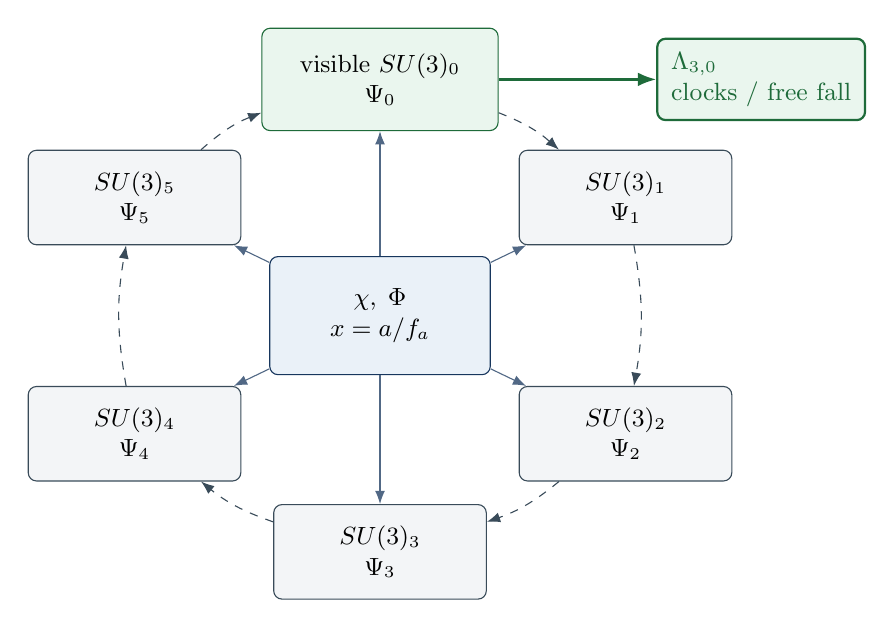
\begin{tikzpicture}[>=Latex, every node/.style={font=\small}]
  \node[draw=navy,fill=lightblue,rounded corners=3pt,minimum width=28mm,minimum height=15mm,align=center] (core) at (0,0) {$\chi,\;\Phi$\\$x=a/f_a$};
  \foreach \k/\ang in {0/90,1/30,2/-30,3/-90,4/-150,5/150}{
    \coordinate (p\k) at ({3.6*cos(\ang)},{3.0*sin(\ang)});
  }
  \node[draw=deepgreen,fill=lightgreen,rounded corners=3pt,minimum width=30mm,minimum height=13mm,align=center] (s0) at (p0) {visible $SU(3)_0$\\$\Psi_0$};
  \foreach \k in {1,...,5}{
    \node[draw=slate,fill=lightgray,rounded corners=3pt,minimum width=27mm,minimum height=12mm,align=center] (s\k) at (p\k) {$SU(3)_{\k}$\\$\Psi_{\k}$};
  }
  \foreach \k in {0,...,5}{
    \draw[->,navy!75] (core) -- (s\k);
  }
  \draw[->,thick,deepgreen] (s0.east) -- ++(2.0,0) node[right,align=left,draw=deepgreen,fill=lightgreen,rounded corners=3pt,inner sep=5pt] {$\Lambda_{3,0}$\\clocks / free fall};
  \draw[->,dashed,slate] (s0) to[bend left=10] (s1);
  \draw[->,dashed,slate] (s1) to[bend left=10] (s2);
  \draw[->,dashed,slate] (s2) to[bend left=10] (s3);
  \draw[->,dashed,slate] (s3) to[bend left=10] (s4);
  \draw[->,dashed,slate] (s4) to[bend left=10] (s5);
  \draw[->,dashed,slate] (s5) to[bend left=10] (s0);
\end{tikzpicture}
\caption{The complete $Z_6$ orbit protects the vacuum potential. Only the highlighted sector contributes to the visible-QCD threshold response.}
\label{fig:architecture}
\end{figure}

\subsection{Exact cyclic symmetry}\label{exact-cyclic-symmetry}

Let

\[
\omega=e^{2\pi i/N}.
\]

The symmetry acts as

\[
\boxed{
\Phi\rightarrow\omega\Phi,
\qquad
\Psi_k\rightarrow\Psi_{k+1},
\qquad
SU(3)_k\rightarrow SU(3)_{k+1}.
}
\]

The renormalizable Yukawa orbit is

\[
\boxed{
\mathcal L_Y
=-\sum_{k=0}^{N-1}
\left[
 y_\chi\chi
-y\left(\omega^k\Phi+\omega^{-k}\Phi^\dagger\right)
\right]
\bar\Psi_k\Psi_k.
}
\]

After radial locking,

\[
M=y_\chi\chi,
\qquad
\epsilon=\frac{\sqrt2yf_a}{M}
=\frac{\sqrt2y\zeta_a}{y_\chi},
\]

and

\[
\boxed{
M_k(a)
=M\left[
1-\epsilon\cos\left(\frac a{f_a}+\frac{2\pi k}{N}\right)
\right].
}
\]

All masses remain strictly positive for

\[
0<\epsilon<1.
\]

Because \(M\propto\chi\) and \(f_a\propto\chi\), \(\epsilon\) is
dimensionless and independent of the common radial scale. The compact
field \(a/f_a\) is therefore a genuine ratio mode.

\subsection{Perturbative health}\label{perturbative-health}

The scalar kinetic term gives

\[
|\partial\Phi|^2
=
\frac12(\partial\rho)^2
+
rac12\left(1+\frac\rho{f_a}\right)^2(\partial a)^2.
\]

Around \(\rho=0\), both kinetic eigenvalues are positive. The radial
mass is

\[
m_\rho^2=2\lambda_\Phi f_a^2>0.
\]

The \(\Psi_k\) are vectorlike, so their colour representations introduce
no chiral gauge anomaly. Each gauge sector is an ordinary local
Yang-Mills theory. The construction therefore avoids the Lorentzian and
spectral difficulties associated with elementary fourth-order fields.

\begin{center}\rule{0.5\linewidth}{0.5pt}\end{center}

\section{All-orders cyclic-protection
theorem}\label{all-orders-cyclic-protection-theorem}

\subsection{Theorem}\label{theorem}

Assume:

\begin{enumerate}
\def\labelenumi{\arabic{enumi}.}
\tightlist
\item
  the complete microscopic action, path-integral measure and regulator
  preserve the cyclic \(Z_N\);
\item
  the limit \(\epsilon\to0\) restores a continuous shift symmetry of
  \(a\);
\item
  the only local shift-breaking spurions are those appearing in the
  complete Yukawa orbit;
\item
  the effective action is analytic in those spurions near
  \(\epsilon=0\).
\end{enumerate}

Then the vacuum effective potential has the form

\[
\boxed{
V_{\rm eff}(a)
=
V_0
+
\sum_{q=1}^{\infty}
\Lambda_q^4
\cos\left(
\frac{qNa}{f_a}+\delta_q
\right),
}
\]

with

\[
\boxed{
\Lambda_q^4=O\left(\epsilon^{qN}\right).
}
\]

In particular, the leading field-dependent term is \(O(\epsilon^N)\).

\subsection{Proof}\label{proof}

The exact exchange symmetry implies

\[
V_{\rm eff}(x)=V_{\rm eff}\left(x+\frac{2\pi}{N}\right).
\]

Its Fourier series can therefore contain only harmonics \(e^{iqNx}\). In
the \(\epsilon=0\) limit, the continuous shift symmetry makes every
nonconstant Fourier coefficient vanish.

Each Yukawa mass insertion supplies one factor of \(\epsilon e^{ix}\) or
\(\epsilon e^{-ix}\). A term proportional to \(e^{iqN x}\) requires at
least \(qN\) net insertions. Hence its coefficient is at least order
\(\epsilon^{qN}\). This argument is independent of loop order. Gauge and
scalar corrections can alter coefficients but cannot create a forbidden
harmonic or reduce the required spurion power.

\subsection{Consequence}\label{consequence}

The dangerous order-\(\epsilon^2\) mass is not balanced against an
unrelated bosonic loop. It is absent because no symmetry-compatible
invariant exists at that order.

\begin{center}\rule{0.5\linewidth}{0.5pt}\end{center}

\section{Explicit one-loop Coleman-Weinberg
potential}\label{explicit-one-loop-coleman-weinberg-potential}

For \(N_c\) colours,

\[
V_{\rm CW}(a)
=-\frac{N_c}{16\pi^2}
\sum_{k=0}^{N-1}
M_k(a)^4
\left[
\ln\frac{M_k(a)^2}{\mu^2}-\frac32
\right].
\]

For \(m<N\), the orbit sums obey

\[
\sum_{k=0}^{N-1}
\cos^m\left(x+\frac{2\pi k}{N}\right)
=
\text{constant in }x.
\]

The first field-dependent identity is

\[
\sum_{k=0}^{N-1}
\cos^N\left(x+\frac{2\pi k}{N}\right)
=
\frac{N}{2^{N-1}}\cos(Nx)+\text{constant}.
\]

For \(N>4\), the divergent and renormalization-scale-dependent terms are
field independent, and expansion of the finite part gives

\[
V_{\rm CW}(a)
=
\frac{N_cM^4\epsilon^N}{8\pi^2}
F_N\cos(Nx)
\left[1+O(\epsilon)\right].
\]

The literature expression

\[
F_N
=
2^{1-N}N
\sum_{\ell=0}^{4}
\binom4\ell\frac{(-1)^\ell}{N-\ell}
\]

simplifies exactly to

\[
\boxed{
F_N
=
\frac{24\,2^{1-N}}
{(N-1)(N-2)(N-3)(N-4)}.
}
\]

At a minimum,

\[
\boxed{
 m_a^2
 =
 \frac{N_cM^4N^2\epsilon^N}{8\pi^2f_a^2}F_N
 \left[1+O(\epsilon)\right]>0.
}
\]

The symmetry statement is all-order; this coefficient is the leading
one-loop realization.

\begin{center}\rule{0.5\linewidth}{0.5pt}\end{center}

\section{\texorpdfstring{Why the visible \(2/27\)
survives}{Why the visible 2/27 survives}}\label{why-the-visible-227-survives}

The partners \(\Psi_{k\ne0}\) cancel the vacuum potential because the
vacuum functional sums over all sectors. They do \textbf{not} enter the
visible QCD beta function because they are not charged under
\(SU(3)_0\).

For our sector, the exact threshold recursion from v0.5 remains

\[
\delta_{n-1}
=A_j\delta_n+(1-A_j)\epsilon_j,
\]

where

\[
\delta_n=\mathrm d\ln\frac{\Lambda_n}{\chi},
\qquad
\epsilon_j=\mathrm d\ln\frac{\widehat m_j}{\chi}.
\]

For the visible threshold chain

\[
7\xrightarrow{\Psi_0}6\xrightarrow{t}5\xrightarrow{b}4\xrightarrow{c}3,
\]

with the Standard Model heavy quarks exactly locked to \(\chi\),

\[
\mathrm d\ln\frac{\Lambda_{3,0}}{\chi}
=\mathcal D_{\Psi\to3}
\mathrm d\ln\frac{M_0}{\chi}.
\]

At one loop,

\[
\begin{aligned}
\mathcal D_{\Psi\to3}^{(1)}
&=
\left(1-\frac{19}{21}\right)
\frac{21}{23}\frac{23}{25}\frac{25}{27}
\\
&=\boxed{\frac{2}{27}}.
\end{aligned}
\]

At higher orders,

\[
\mathcal D_{\Psi\to3}
=\frac{2}{27}+O(\alpha_s(M)),
\]

with corrections calculable from standard decoupling functions.

For a general background \(x_0=a_0/f_a\), define

\[
\kappa_0
\equiv
\frac{\partial}{\partial x}
\ln\frac{M_0}{\chi}
\bigg|_{x_0}
=
\frac{\epsilon\sin x_0}{1-\epsilon\cos x_0}.
\]

Then

\[
\boxed{
\frac{\partial}{\partial a}
\ln\frac{\Lambda_{3,0}}{\chi}
=
\left[\frac{2}{27}+O(\alpha_s)\right]
\frac{\kappa_0}{f_a}.
}
\]

This is the key decoupling:

\[
\kappa_0=O(\epsilon),
\qquad
m_a^2=O(\epsilon^N).
\]

\begin{center}\rule{0.5\linewidth}{0.5pt}\end{center}

\section{\texorpdfstring{Minimal working benchmark:
\(Z_6\)}{Minimal working benchmark: Z\_6}}\label{minimal-working-benchmark-z_6}

For \(N=6\),

\[
F_6=\frac1{160}.
\]

The potential has six minima

\[
x_m=\frac{(2m-1)\pi}{6}.
\]

Choose the symmetry-related vacuum

\[
\boxed{x_0=\frac\pi2.}
\]

Then

\[
\cos x_0=0,
\qquad
\sin x_0=1,
\]

so

\[
M_0=M,
\qquad
\boxed{\kappa_0=\epsilon.}
\]

For \(N_c=3\),

\[
\boxed{
V_{\rm CW}^{(6)}
=
\frac{3M^4\epsilon^6}{1280\pi^2}
\cos\left(\frac{6a}{f_a}\right)
+O(\epsilon^7),
}
\]

and

\[
\boxed{
 m_a^2
 =
 \frac{27}{320\pi^2}
 \frac{M^4}{f_a^2}\epsilon^6
 +O(\epsilon^7).
}
\]

The QCD coupling is

\[
\boxed{
 d_g
 =
 \frac{2}{27}\frac{M_{\rm P}}{f_a}\epsilon
 +O(\alpha_s\epsilon,\epsilon^2).
}
\]

Eliminating \(\epsilon\) gives the model's mass-coupling protection law:

\[
\boxed{
\frac{m_a^2f_a^2}{M^4}
=
\frac{27}{320\pi^2}
\left(
\frac{27}{2}\frac{f_a}{M_{\rm P}}d_g
\right)^6
+\cdots.
}
\]

This is the central quantitative gain: the coupling enters the radiative
mass at sixth order rather than second order.

\subsection{Numerical illustration}\label{numerical-illustration}

Take

\[
M=10\ \mathrm{TeV},
\qquad
f_a=M_{\rm P}=2.435\times10^{18}\ \mathrm{GeV}.
\]

\begin{longtable}[]{@{}
  >{\raggedleft\arraybackslash}p{(\columnwidth - 8\tabcolsep) * \real{0.2000}}
  >{\raggedleft\arraybackslash}p{(\columnwidth - 8\tabcolsep) * \real{0.2000}}
  >{\raggedleft\arraybackslash}p{(\columnwidth - 8\tabcolsep) * \real{0.2000}}
  >{\raggedleft\arraybackslash}p{(\columnwidth - 8\tabcolsep) * \real{0.2000}}
  >{\raggedleft\arraybackslash}p{(\columnwidth - 8\tabcolsep) * \real{0.2000}}@{}}
\toprule\noalign{}
\begin{minipage}[b]{\linewidth}\raggedleft
\(N\)
\end{minipage} & \begin{minipage}[b]{\linewidth}\raggedleft
\(\epsilon\)
\end{minipage} & \begin{minipage}[b]{\linewidth}\raggedleft
\(d_g\) at maximal slope
\end{minipage} & \begin{minipage}[b]{\linewidth}\raggedleft
\(m_a\)
\end{minipage} & \begin{minipage}[b]{\linewidth}\raggedleft
Compton range
\end{minipage} \\
\midrule\noalign{}
\endhead
\bottomrule\noalign{}
\endlastfoot
5 & \(10^{-6}\) & \(7.41\times10^{-8}\) & \(1.00\times10^{-17}\) eV &
\(0.132\) AU \\
6 & \(10^{-6}\) & \(7.41\times10^{-8}\) & \(3.80\times10^{-21}\) eV &
\(347\) AU \\
8 & \(10^{-6}\) & \(7.41\times10^{-8}\) & \(9.57\times10^{-28}\) eV &
\(1.38\times10^9\) AU \\
6 & \(10^{-3}\) & \(7.41\times10^{-5}\) & \(3.80\times10^{-12}\) eV &
\(3.47\times10^{-7}\) AU \\
\end{longtable}



\begin{figure}[H]
\centering
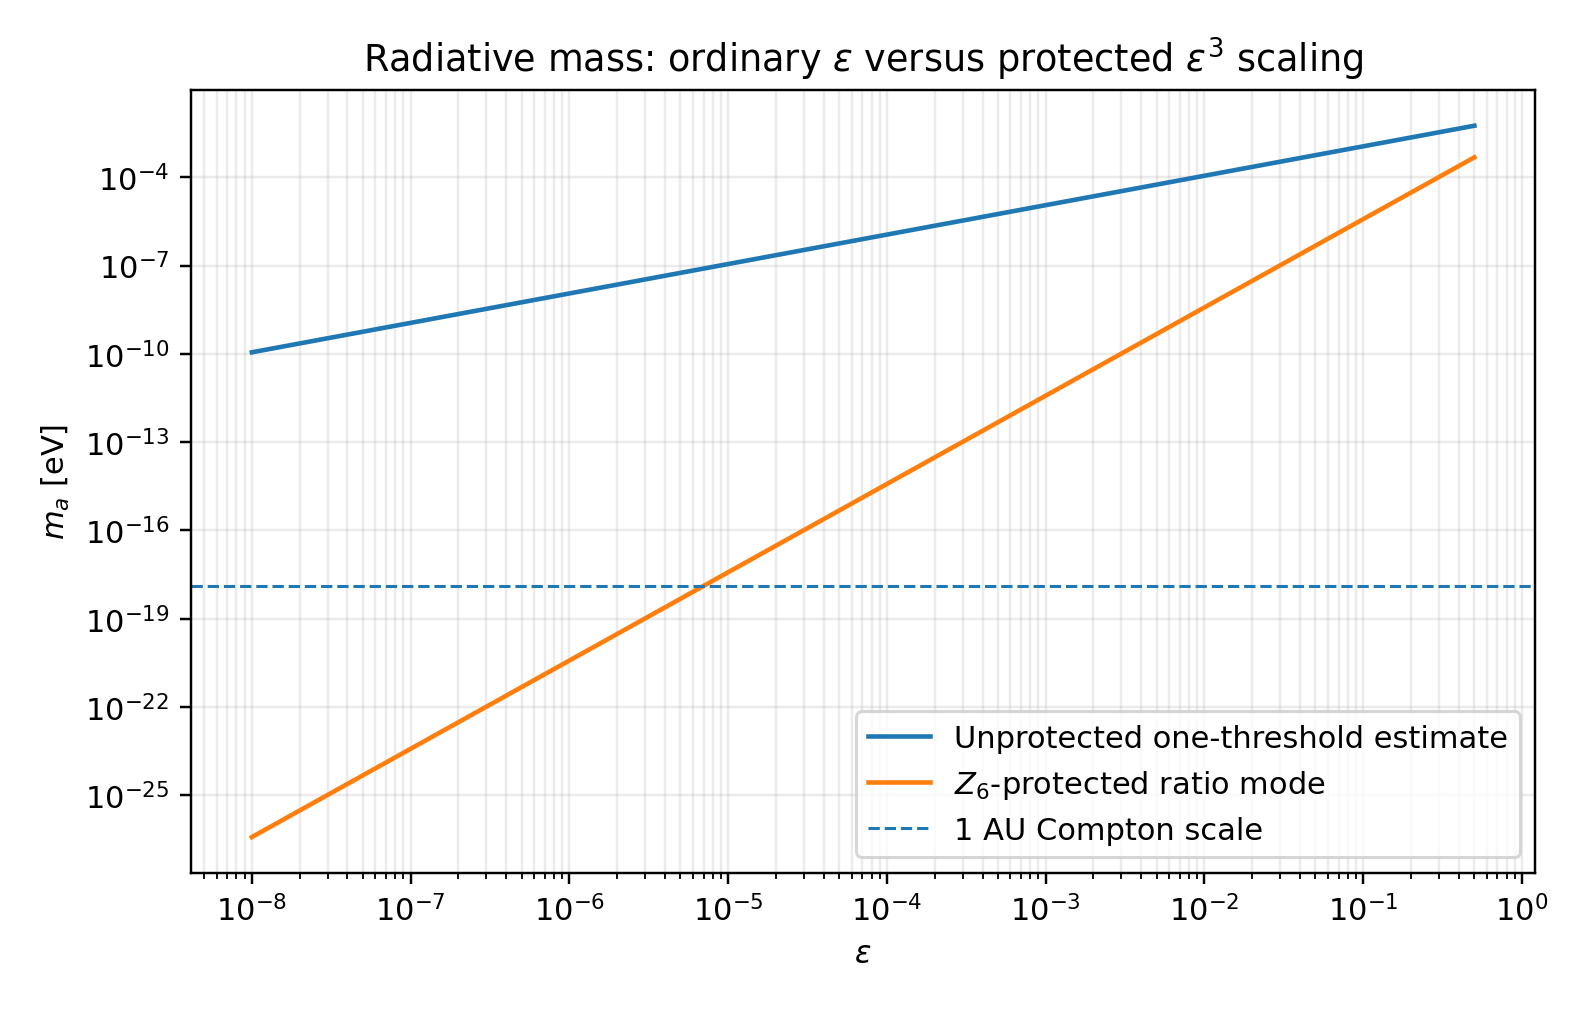
\includegraphics[width=0.88\textwidth]{zn_protected_mass_scaling_v0_6.png}
\caption{One-loop mass scaling for $M=10$ TeV and $f_a=M_{\rm P}$. The unprotected mode scales as $m_a\propto\epsilon$, whereas the $Z_6$ mode scales as $m_a\propto\epsilon^3$.}
\label{fig:massscaling}
\end{figure}

For the \(N=6,\epsilon=10^{-6}\) point, the ordinary unprotected
estimate is

\[
m_{a,\rm naive}\simeq1.13\times10^{-8}\ \mathrm{eV},
\]

whereas the protected result is

\[
m_{a,Z_6}\simeq3.80\times10^{-21}\ \mathrm{eV}.
\]

The squared-mass suppression is

\[
\frac{m_{a,Z_6}^2}{m_{a,\rm naive}^2}
=1.125\times10^{-25}.
\]

\begin{center}\rule{0.5\linewidth}{0.5pt}\end{center}

\section{Chronometric and equivalence-principle
predictions}\label{chronometric-and-equivalence-principle-predictions}

The protection changes the naturalness relation; it does not erase the
low-energy prediction derived in v0.5.

For clock transitions \(A\) and \(B\),

\[
\mathcal S_{AB}
\equiv
\mathrm d\ln\frac{\nu_A}{\nu_B}.
\]

In the pure-QCD benchmark,

\[
\boxed{
\mathcal S_{AB}
=
(\Delta K_\mu-\Delta K_q)
\frac{2}{27}\kappa_0\,\mathrm dx
+\cdots.
}
\]

At the \(Z_6\) benchmark vacuum, \(\kappa_0=\epsilon\), so

\[
\boxed{
\mathcal S_{AB}
=
(\Delta K_\mu-\Delta K_q)
\frac{2\epsilon}{27}\frac{\mathrm da}{f_a}
+\cdots.
}
\]

The rank-one relation remains

\[
\boxed{
\mathcal S_{\rm Sr/Cs}
=2\mathcal S_{\rm Sr/CaF}
}
\]

under the same leading sensitivity assumptions used in v0.5.

For one unscreened scalar and one dominant QCD spurion, the
clock--equivalence-principle consistency line also remains

\[
\boxed{
\frac{\beta_{AB}}{\eta_{CD}}
=-
\frac{\Delta K_\mu-\Delta K_q}
{\Delta Q'_{\widehat m}{}^{CD}}.
}
\]

The \(Z_N\) sector changes the technically natural relation between
\(m_a\) and the common coupling \(d_g\); the coupling cancels from the
dimensionless clock/EP ratio.

\begin{center}\rule{0.5\linewidth}{0.5pt}\end{center}

\section{Exact symmetry requirements and failure
modes}\label{exact-symmetry-requirements-and-failure-modes}

\subsection{The complete renormalization environment must be
replicated}\label{the-complete-renormalization-environment-must-be-replicated}

It is not enough to add \(N-1\) arbitrary spectator fermions. If
\(\Psi_0\) interacts with visible QCD while its partners see different
gauge or matter content, gauge corrections split their masses and Yukawa
functions. That splitting is a hard \(Z_N\)-breaking spurion and
regenerates low harmonics.

The safe microscopic options are:

\begin{enumerate}
\def\labelenumi{\arabic{enumi}.}
\tightlist
\item
  replicate the full Standard Model, as in existing \(Z_N\)-protected
  modulus constructions;
\item
  replicate at least every gauge and matter interaction entering the
  \(\Psi_k\) renormalization functions;
\item
  derive the exchange symmetry from a discrete gauge or geometric
  translation symmetry.
\end{enumerate}

\subsection{Quantitative tolerance to hard
breaking}\label{quantitative-tolerance-to-hard-breaking}

Let sector-dependent corrections be represented by weights
\(1+\Delta_k\). Define their discrete Fourier components

\[
\widetilde\Delta_p
=\frac1N\sum_{k=0}^{N-1}
\Delta_k e^{-2\pi ipk/N}.
\]

An order-\(p\) harmonic can then appear parametrically as

\[
\delta V_p
\sim
\frac{N_cM^4}{16\pi^2}
\widetilde\Delta_p\epsilon^p
\cos(px+\delta_p).
\]

For the protected \(N\)-th harmonic to dominate,

\[
\boxed{
|\widetilde\Delta_p|
\lesssim
\epsilon^{N-p},
\qquad p<N,
}
\]

up to order-one coefficient ratios.

For \(N=6\) and \(\epsilon=10^{-6}\), this is ferocious. The symmetry
must be exact in the Lagrangian; approximate sector equality is not
enough.

\subsection{Elementary-field quality
problem}\label{elementary-field-quality-problem}

The operator

\[
\frac{c_N}{M_*^{N-4}}
\left(\Phi^N+\Phi^{\dagger N}\right)
\]

is allowed by \(Z_N\). It produces

\[
\delta m_a^2
\sim
N^2|c_N|
\frac{f_a^{N-2}}{M_*^{N-4}}.
\]

For a high decay constant, this can overwhelm the protected fermion-loop
potential. Therefore the elementary-global-\(\Phi\) theory is an
infrared model, not a sufficient ultraviolet explanation.

A credible completion must make the approximate continuous shift a gauge
or geometric remnant, or otherwise suppress \(c_N\) by a controlled
microscopic mechanism.

\begin{center}\rule{0.5\linewidth}{0.5pt}\end{center}

\section{Preferred quality completion: a deconstructed Wilson-line ratio
mode}\label{preferred-quality-completion-a-deconstructed-wilson-line-ratio-mode}

The most attractive ultraviolet direction is to realize \(a\) as the
gauge-invariant Wilson-line phase of a four-dimensional deconstructed
gauge theory.

Take a cyclic moose of gauge groups connected by link scalars. Local
gauge transformations remove all but one collective phase. The remaining
gauge-invariant variable is schematically

\[
\exp\left(i\frac a{f_a}\right)
\sim
\prod_j\frac{\Sigma_j}{|\Sigma_j|}.
\]

Its shift symmetry descends from gauge invariance. Local renormalizable
operators cannot depend on the full Wilson loop; an \(a\)-dependent
potential requires propagation around the complete theory-space circle
or explicit boundary/nonlocal breaking. This supplies:

\begin{itemize}
\tightlist
\item
  a discrete/geometric origin for the cyclic exchange;
\item
  protection against generic local ultraviolet operators;
\item
  a natural explanation for why the first field-dependent invariant
  requires a complete orbit;
\item
  a route to a fully renormalizable four-dimensional quality completion.
\end{itemize}

A complete model must still derive the separate-QCD-sector mass orbit
while keeping the colour groups distinct. The technically clean
implementation is a replicated colour quiver linked only through a
gauge-protected singlet Wilson-line sector and symmetry-related
messenger chains. This is a concrete next construction rather than a
solved detail of the present note.

\begin{center}\rule{0.5\linewidth}{0.5pt}\end{center}

\section{Cosmological and environmental
issues}\label{cosmological-and-environmental-issues}

\subsection{Mirror sectors and
reheating}\label{mirror-sectors-and-reheating}

Exact microscopic \(Z_N\) implies degenerate sectors. If all are
reheated equally, hidden radiation and relics are generally
unacceptable. The symmetry should be broken by the \textbf{state}, not
by hard couplings:

\[
\text{exact symmetric Lagrangian}
+\text{asymmetric initial condition/reheating state}.
\]

A reheating model must preserve the ultraviolet cancellation while
populating primarily one sector. Recent cyclic models explicitly exploit
spontaneous asymmetry of the relic state while retaining exact
microscopic symmetry.

\subsection{Finite-density potential}\label{finite-density-potential}

Visible matter is itself a sector-asymmetric state. It generates

\[
V_{\rm matter}(a)
=\rho_{\rm vis}
\left[
1+\alpha_{\rm vis}\frac{a-a_0}{M_{\rm P}}+\cdots
\right].
\]

This term is not \(\epsilon^N\)-suppressed. It is the physical source of
the fifth force and clock redshift, but it can also:

\begin{itemize}
\tightlist
\item
  shift the local vacuum;
\item
  increase the in-medium effective mass;
\item
  screen or pin the field inside dense bodies;
\item
  create nontrivial boundary profiles between sectors of different
  density.
\end{itemize}

The next phenomenological calculation must solve the nonlinear static
field profile for Earth, Sun and laboratory source geometries.

\subsection{Domain walls}\label{domain-walls}

The protected vacuum has \(N\) degenerate minima. Domain walls are
avoided if:

\begin{itemize}
\tightlist
\item
  symmetry breaking occurs before inflation and is not thermally
  restored;
\item
  a tiny symmetry-compatible bias removes the degeneracy without
  spoiling the mass hierarchy;
\item
  or the discrete symmetry is gauged/geometric so apparently distinct
  vacua are identified appropriately.
\end{itemize}

\subsection{Heavy coloured fermions}\label{heavy-coloured-fermions}

A stable visible colour triplet is excluded cosmologically. The visible
\(\Psi_0\) must decay. A vectorlike down-type or up-type assignment with
small replicated mixing can provide decays while preserving the one-loop
fundamental-representation threshold coefficient. The exact collider
bound is decay-model dependent and is not fixed in this note.

\subsection{CP structure}\label{cp-structure}

The mass orbit is real. Integrating out \(\Psi_k\) produces
\(aG_k^{\mu\nu}G^k_{\mu\nu}\)-type scalar couplings, not an anomalous
\(aG\widetilde G\) term from a complex fermion mass phase. A generalized
CP assignment and the chosen vacuum must nevertheless be specified in a
full phenomenological model.

\begin{center}\rule{0.5\linewidth}{0.5pt}\end{center}

\section{Novelty boundary}\label{novelty-boundary}

The broad protection mechanism is established:

\begin{itemize}
\tightlist
\item
  nonlinearly realized discrete symmetries can permit nonderivative
  Yukawa couplings while forcing the radiative potential to begin at
  high spurion order;
\item
  replicated-Standard-Model \(Z_N\) models have used the same orbit
  cancellation to keep a photon-coupled modulus ultralight;
\item
  mirror-QCD \(Z_N\) constructions suppress axion masses while
  preserving comparatively large couplings;
\item
  a 2026 axion--WIMP model again uses cyclic fermions to project the
  Coleman-Weinberg potential onto the \(N\)-th harmonic.
\end{itemize}

Therefore the following cannot be claimed as new:

\[
\text{``use }Z_N\text{ copies to obtain }V\sim\epsilon^N\text{ while a one-sector coupling is }O(\epsilon).''
\]

The candidate original contribution is narrower:

\begin{enumerate}
\def\labelenumi{\arabic{enumi}.}
\tightlist
\item
  a \textbf{CP-even vectorlike QCD threshold} rather than a photon
  threshold or anomalous axion coupling;
\item
  preservation of the exact visible-QCD decoupling response \[
  \mathcal D_{\Psi\to3}^{(1)}=\frac{2}{27};
  \]
\item
  embedding that response in the universal-scale-lock/chronometric-shear
  framework;
\item
  the \(Z_6\) mass--coupling law \[
  m_a^2\propto d_g^6;
  \]
\item
  the observation that cyclic protection leaves the dimensionless
  clock--EP consistency line unchanged while making an ultralight
  mediator technically possible.
\end{enumerate}

A systematic priority search found close precedents for every mechanism,
but no exact indexed match for this combined QCD-threshold/chronometric
construction. That remains a candidate priority claim, not a declaration
of priority.

\begin{center}\rule{0.5\linewidth}{0.5pt}\end{center}

\section{What has been solved and what has
not}\label{what-has-been-solved-and-what-has-not}

\subsection{Solved in this step}\label{solved-in-this-step}

\[
\boxed{
\begin{gathered}
\text{exact cyclic symmetry}
\Longrightarrow
V_{\rm vac}(a)=O(\epsilon^N),\\[1mm]
\text{one visible fundamental threshold}
\Longrightarrow
\mathrm d\ln(\Lambda_3/\chi)
=\frac{2}{27}\mathrm d\ln(M_0/\chi)+\cdots,\\[1mm]
N=6,\ x_0=\pi/2
\Longrightarrow
m_a^2=\frac{27}{320\pi^2}\frac{M^4}{f_a^2}\epsilon^6,
\quad
d_g=\frac{2}{27}\frac{M_{\rm P}}{f_a}\epsilon.
\end{gathered}
}
\]

This removes the catastrophic \(M^4\epsilon^2/f_a^2\) contribution
without nullifying the desired QCD response.

\subsection{Still open}\label{still-open}

\begin{enumerate}
\def\labelenumi{\arabic{enumi}.}
\tightlist
\item
  construct the full discrete-gauge/deconstructed messenger completion
  that produces the orbit while keeping \(SU(3)_k\) sectors distinct;
\item
  derive two-loop gauge/Yukawa corrections and verify the
  \(O(\epsilon^N)\) spurion counting in the complete replicated theory;
\item
  solve asymmetric reheating without hard \(Z_N\) breaking;
\item
  calculate finite-density screening around realistic sources;
\item
  specify the decaying vectorlike-quark phenomenology;
\item
  combine current clock, MICROSCOPE, torsion-balance, stellar and
  cosmological limits in one likelihood;
\item
  test whether the same protection can arise from the proposed deeper
  36-field/Turok sector rather than an added elementary \(\Phi\).
\end{enumerate}

\begin{center}\rule{0.5\linewidth}{0.5pt}\end{center}

\section{Immediate next calculation}\label{immediate-next-calculation}

The next decisive calculation is no longer the vacuum mass. It is the
\textbf{environmental field profile}.

For the \(Z_6\) benchmark, derive and solve

\[
\Box a
=
\frac{\partial V_{Z_6}}{\partial a}
+\sum_A
\frac{\partial\ln m_A(a)}{\partial a}\rho_A(x)
\]

for spherical sources, including the QCD composition charges of Earth,
Sun and laboratory test bodies. This will determine whether the same
finite-density effect that makes the model observable also screens it.

A parallel ultraviolet task is to construct the deconstructed
gauge-quality completion and compute its leading nonlocal breaking
operator. Those two tasks now dominate the viability question.

\begin{center}\rule{0.5\linewidth}{0.5pt}\end{center}

\section{References}\label{references}

\begin{enumerate}
\def\labelenumi{\arabic{enumi}.}
\tightlist
\item
  S. Das and A. Hook, \emph{Non-linearly realized discrete symmetries},
  arXiv:2006.10767.
\item
  D. Brzeminski, Z. Chacko, A. Dev and A. Hook, \emph{A Time-Varying
  Fine Structure Constant from Naturally Ultralight Dark Matter}, Phys.
  Rev.~D 104, 075019 (2021), arXiv:2012.02787.
\item
  L. Di Luzio, B. Gavela, P. Quilez and A. Ringwald, \emph{An even
  lighter QCD axion}, JHEP 05 (2021) 184, arXiv:2102.00012.
\item
  C. Delaunay, S. J. Lee, Y. Yin and B. Yu, \emph{Natural Phantom
  Crossing from Axion-WIMP Interactions}, arXiv:2607.28721.
\item
  S. Hor, Y. Nakai, M. Suzuki and J. Xu, \emph{Deconstructing the
  Extra-Dimensional Axion}, arXiv:2606.02728.
\item
  K. G. Chetyrkin, B. A. Kniehl and M. Steinhauser, \emph{Decoupling
  relations to O(alpha\_s\^{}3) and their connection to low-energy
  theorems}, Nucl. Phys. B 510 (1998) 61, arXiv:hep-ph/9708255.
\item
  T. Damour and J. F. Donoghue, \emph{Equivalence principle violations
  and couplings of a light dilaton}, Phys. Rev.~D 82, 084033 (2010),
  arXiv:1007.2792.
\item
  P. Touboul et al., \emph{MICROSCOPE Mission: Final Results of the Test
  of the Equivalence Principle}, Phys. Rev.~Lett. 129, 121102 (2022),
  arXiv:2209.15487.
\end{enumerate}

\begin{center}\rule{0.5\linewidth}{0.5pt}\end{center}

\section{Verification statement}\label{verification-statement}

The accompanying verification script independently checks:

\begin{itemize}
\tightlist
\item
  the closed form of \(F_N\);
\item
  root-of-unity cancellation for \(m<N\);
\item
  the numerical one-loop Fourier coefficient for representative \(N\);
\item
  the telescoping \(2/27\) threshold coefficient;
\item
  the exact \(Z_6\) identities \(F_6=1/160\), \(\kappa_0=\epsilon\) and
  \(m_a^2=(27/320\pi^2)M^4\epsilon^6/f_a^2\);
\item
  positivity of all \(M_k\) over 100,000 random points with
  \(0<\epsilon<1\);
\item
  representative mass/range benchmarks.
\end{itemize}

All programmed checks pass.

\end{document}
